\documentclass[12pt,fleqn]{article}
\usepackage{
  amsmath,
  amssymb,
  booktabs,
  geometry,
  graphicx,
  microtype,
  parskip,
  caption,
}
\usepackage[shortlabels]{enumitem}

\geometry{margin=3cm}

% equation line spacing
\setlength{\jot}{0.5cm}

% meta data
\newcommand{\chapter}{6.5}
\newcommand{\authorname}{Amo DelBello}
\newcommand{\classdescription}{MATH 1350-D2}
\newcommand{\classname}{Introduction to Statistics, Fall 2022}
\newcommand{\assignment}{\chapter\ Book Assignment}

\newcommand{\problem}[1]{\vspace{5ex}\section*{\chapter-#1}}
\newcommand{\thead}[1]{\textnormal{\textbf{#1}}}
\newcommand{\tvspace}{\vspace{.25cm}}

\title{\classdescription\ \\ \classname\ \\ $\ $ \\ \assignment}
\author{\authorname}
\date{\today}


\begin{document}

\maketitle


\problem{9}
The histogram of the Chips Ahoy Reduced Fat cookies, while not perfect, appears to be roughly normal.


\problem{13}
\begin{figure}[ht]
  \centering
  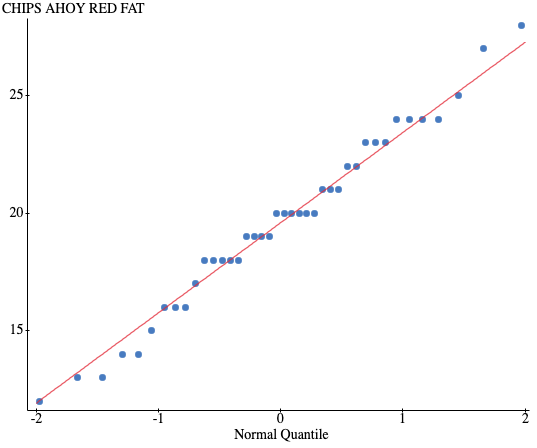
\includegraphics[width=8cm]{assets/cookies-qq.png}
\end{figure}
The data appears to be normally distributed.


\problem{17}
Data set (cm): 40.7, 44.3, 34.2, 32.5, 38.5

\begin{enumerate}
\item \textbf{Sort the data}: 32.5, 34.2, 38.5, 40.7, 44.3

\item \textbf{Find the $n$ values}:
  $n = 5$, $\frac{1}{2n} \text{, } \frac{3}{2n} \text{, } \frac{5}{2n} \text{, } \frac{7}{2n} \text{, } \frac{9}{2n}$

  $\frac{1}{10} \text{, } \frac{3}{10} \text{, } \frac{5}{10} \text{, } \frac{7}{10} \text{, } \frac{9}{10} \text{, } $

\item \textbf{Use the standard normal distribution to find the \textit{z scores}}:

  -1.28, -0.52, 0, 0.52, 1.28

\item \textbf{Match the original sorted data values with their corresponding $z$ scores}:

  (32.5, -1.28), (34.2, -0.52), (38.5, 0), (40.7, 0.52), (44.3, 1.28)

\item \textbf{Examine the normal quantile plot and determine if distribution is normal}:

Although there aren't that many data points, they do appear to be loosely normal.
\begin{figure}[ht]
  \centering
  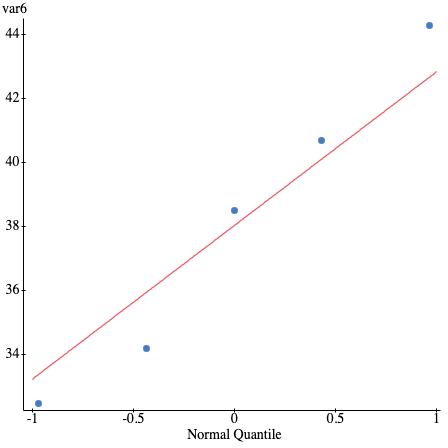
\includegraphics[width=8cm]{assets/female-arms.png}
\end{figure}
\end{enumerate}


\problem{19}
Data set: 1027, 1029, 1034, 1070, 1079, 1079, 963, 1439

\begin{enumerate}
\item \textbf{Sort the data}: 963, 1027, 1029, 1034, 1070, 1079, 1079, 1439

\item \textbf{Find the $n$ values}:
$n = 8$,
  $\frac{1}{2n} \text{, }
  \frac{3}{2n} \text{, }
  \frac{5}{2n} \text{, }
  \frac{7}{2n} \text{, }
  \frac{9}{2n} \text{, }
  \frac{11}{2n} \text{, }
  \frac{13}{2n} \text{, }
  \frac{15}{2n}$

  $\frac{1}{16} \text{, }
  \frac{3}{16} \text{, }
  \frac{5}{16} \text{, }
  \frac{7}{16} \text{, }
  \frac{9}{16} \text{, }
  \frac{11}{16} \text{, }
  \frac{13}{16} \text{, }
  \frac{15}{16} \text{, } $

\item \textbf{Use the standard normal distribution to find the \textit{z scores}}:

-1.53, -0.89, -0.49, -0.16, 0.16, 0.49, 0.89, 1.53

\item \textbf{Match the original sorted data values with their corresponding $z$ scores}:

(963, -1.53), (1027, -0.89), (1029, -0.49), (1034, -0.16), (1070, 0.16), (1079, 0.49), (1079, 0.89), (1439, 1.53)

\item \textbf{Examine the normal quantile plot and determine if distribution is normal}:

The data does not appear to be normal.
\begin{figure}[ht]
  \centering
  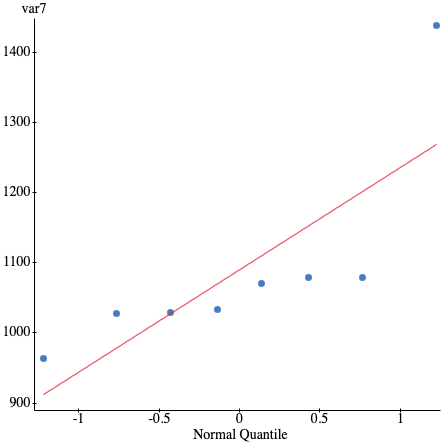
\includegraphics[width=8cm]{assets/brains.png}
\end{figure}
\end{enumerate}


\pagebreak
\problem{20}
Data set: 84, 121, 119, 146, 266, 181, 123, 152, 162

\begin{enumerate}
\item \textbf{Sort the data}: 84, 119, 121, 123, 146, 152, 162, 181, 266

\item \textbf{Find the $n$ values}:
  $n = 9$,
  $\frac{1}{2n} \text{, }
  \frac{3}{2n} \text{, }
  \frac{5}{2n} \text{, }
  \frac{7}{2n} \text{, }
  \frac{9}{2n} \text{, }
  \frac{11}{2n} \text{, }
  \frac{13}{2n} \text{, }
  \frac{15}{2n} \text{, }
  \frac{17}{2n}$

  $\frac{1}{18} \text{, }
  \frac{3}{18} \text{, }
  \frac{5}{18} \text{, }
  \frac{7}{18} \text{, }
  \frac{9}{18} \text{, }
  \frac{11}{18} \text{, }
  \frac{13}{18} \text{, }
  \frac{15}{18} \text{, }
  \frac{17}{18} \text{, } $

\item \textbf{Use the standard normal distribution to find the \textit{z scores}}:

-1.59, -0.97, -0.59, -0.28, 0, 0.28, 0.59, 0.97, 1.59

\item \textbf{Match the original sorted data values with their corresponding $z$ scores}:

(84, -1.59), (119, -0.97), (121, -0.59), (123, -0.28), (146, 0), (152, 0.28), (162, 0.59), (181, 0.97), (266, 1.59)

\item \textbf{Examine the normal quantile plot and determine if distribution is normal}:

There is a single outlier, but otherwise the data appears to be loosely normal.
\begin{figure}[ht]
  \centering
  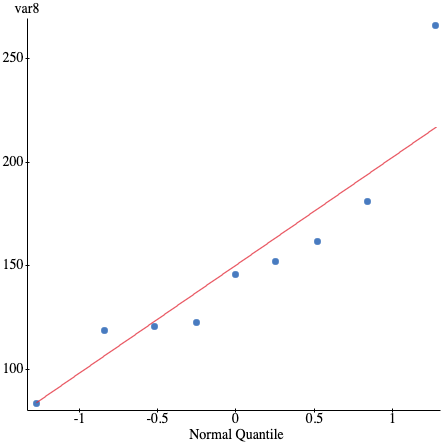
\includegraphics[width=8cm]{assets/fast-food.png}
\end{figure}
\end{enumerate}


\end{document}
%%% Local Variables:
%%% mode: latex
%%% TeX-master: t
%%% End:
